\documentclass[10pt,a4paper,twocolumn]{article}
\usepackage[top=1.8cm,bottom=1.9cm,left=1.7cm,right=1.7cm,columnsep=0.65cm]{geometry}
\usepackage[utf8]{inputenc}
\usepackage[T1]{fontenc}
\usepackage[provide=*,italian]{babel}
\usepackage{amsmath,amssymb,amsthm,mathtools,bm}
\usepackage{mathptmx,microtype}
\usepackage{booktabs,array,tabularx,graphicx,xcolor}
\usepackage{tikz}
\usetikzlibrary{calc}
\usepackage{caption}
\captionsetup{font=small,labelfont=bf,justification=justified,singlelinecheck=false}
\captionsetup[table]{skip=5pt}
\usepackage{placeins,stfloats,float}
\usepackage[numbers,sort&compress]{natbib}
\usepackage[colorlinks=true,linkcolor=blue!40!black,citecolor=blue!40!black,urlcolor=blue!40!black]{hyperref}
\usepackage[nameinlink,noabbrev]{cleveref}
\newtheorem{proposition}{Proposizione}[section]
\newtheorem{theorem}[proposition]{Teorema}
\newtheorem{lemma}[proposition]{Lemma}
\newcommand{\R}{\mathbb{R}}
\newcommand{\norm}[1]{\left\lVert #1\right\rVert}
\emergencystretch=1.5em
\allowdisplaybreaks[1]
\setlength{\tabcolsep}{4pt}
\renewcommand{\arraystretch}{1.15}
\renewcommand{\topfraction}{0.90}
\renewcommand{\bottomfraction}{0.80}
\renewcommand{\dbltopfraction}{0.90}
\renewcommand{\textfraction}{0.08}
\renewcommand{\floatpagefraction}{0.75}
\renewcommand{\dblfloatpagefraction}{0.75}
\setcounter{topnumber}{3}\setcounter{bottomnumber}{2}\setcounter{totalnumber}{5}\setcounter{dbltopnumber}{3}
\setlength{\textfloatsep}{11pt plus 2pt minus 2pt}
\setlength{\dbltextfloatsep}{11pt plus 2pt minus 2pt}
\setlength{\floatsep}{9pt plus 2pt minus 2pt}
\setlength{\dblfloatsep}{9pt plus 2pt minus 2pt}
\raggedbottom

\title{Parallelizzazione della Continuous Particle Swarm Optimization: semantiche di esecuzione, topologie e protocolli di valutazione}
\author{
  \textbf{Giovanni Giuseppe Iacuzzo}\textsuperscript{1,*} \\
  \small \textsuperscript{1}Dipartimento di Ingegneria e Architettura, Universit\`a degli Studi di Enna ``Kore'', Enna, Italia \\
  \small \textsuperscript{*}Autore corrispondente: \texttt{giovanni.iacuzzo@unikore.it}
}
\date{}
\begin{document}
\maketitle
\begin{abstract}
La parallelizzazione della Particle Swarm Optimization modifica non soltanto il costo delle valutazioni, ma potenzialmente anche la semantica dell'aggiornamento sociale e, quindi, le traiettorie di ricerca. Questo lavoro sviluppa un protocollo di studio per la formulazione continua di Orlando--Ricciardello, basata sulla propagazione analitica locale di un sistema differenziale a coefficienti congelati. Si distinguono esecutori sincroni che preservano l'ordine dei commit, un esecutore asincrono a eventi e un modello a isole con migrazione controllata. Il disegno prevede una selezione del passo temporale su problemi e semi appaiati, seguita dalla validazione indipendente del candidato congelato; confronti di tempo assoluto, accelerazione rispetto al seriale, strong scaling ed efficienza; e analisi della qualità al variare delle otto configurazioni di vicinato. Una seconda linea sperimentale definisce un confronto a budget di valutazioni uniforme con dieci varianti PSO su COCO BBOB, BBOB-LargeScale e CEC 2013 LSGO. Vengono precisati l'unit\`a statistica, i confondenti della misura dei tempi e i limiti inferenziali di confronti a parit\`a di valutazioni anzich\'e di tempo. Il contributo attuale \`e la specificazione matematica e metodologica di un quadro di valutazione verificabile, senza anticipare esiti delle campagne ancora da consolidare.
\end{abstract}
\noindent\textbf{Parole chiave:} Continuous Particle Swarm Optimization; parallelismo multicore; propagatore analitico; topologie sociali; strong scaling; benchmarking.

\section{Introduzione}\label{sec:introduction}
\section{Introduzione}
\label{sec:introduction}

La Continuous Particle Swarm Optimization (CPSO) descrive il moto di ciascuna particella mediante un problema di Cauchy del secondo ordine \citep{orlando2020analytic}. La soluzione analitica su ciascun intervallo definisce un aggiornamento dipendente dalla durata del passo e dagli attrattori individuali e sociali. Il passo regola sia la contrazione del moto sia la fase delle oscillazioni. La scelta del suo valore modifica quindi la ricerca anche a parità di valutazioni.

L'esecuzione multicore introduce una seconda variabile. Con aggiornamenti sincroni il lavoro per particella può essere distribuito mantenendo la sequenza dei punti valutati. Con aggiornamenti asincroni, la disponibilità anticipata di un risultato modifica anche l'informazione usata dalle altre particelle. Per valutare questi effetti occorrono confronti appaiati che distinguano tempo di calcolo, qualità a parità di valutazioni e qualità entro una scadenza.

Il lavoro valuta la sensibilità al passo su sei funzioni e verifica la scelta su un campione indipendente. Misura poi la scalabilità sincrona su Rastrigin e su un problema di diffusione inversa, variando il costo della valutazione e il numero di unità di esecuzione (emph{worker}). Infine, confronta il CPSO con un controllo discreto abbinato e con varianti PSO di letteratura. Il controllo abbinato isola l'effetto della legge di aggiornamento. I benchmark a tempo fissato stabiliscono se l'aumento della capacità di valutazione si traduca in un raggiungimento anticipato del target.

\FloatBarrier
\section{Stato dell'arte e posizionamento}
\label{sec:related-work}

\subsection{Dal sistema dinamico discreto alla propagazione continua}
L'evoluzione della PSO \`e stata studiata mediante modelli dinamici, analisi di stabilit\`a e regole di controllo dell'inerzia \citep{ShiEberhart1998,Clerc2002,FernandezMartinezGarciaGonzalo2009,FernandezMartinezGarciaGonzalo2011}. Modelli continui sono stati proposti anche da Emara e Abdel Fattah e da Fern\'andez-Mart\'inez e Garc\'ia-Gonzalo \citep{Emara2004,FernandezMartinezGarciaGonzalo2008}. Orlando e Ricciardello impiegano un problema di Cauchy lineare a coefficienti localmente costanti per definire la CPSO \citep{Orlando2021}. Il presente lavoro adotta questa famiglia di dinamiche, specificando le convenzioni numeriche necessarie a confrontare modalit\`a di esecuzione differenti. In assenza di una dimostrazione specifica non si estendono alla traiettoria complessiva le propriet\`a della sola soluzione locale.

La lettura stocastica e di campo medio della PSO offre un punto di vista complementare sulla dinamica collettiva \citep{GrassiPareschi2021}; le rassegne sui sistemi a sciame chiariscono il ruolo di parametri, vincoli e strutture sociali \citep{BonyadiMichalewicz2017}. Qui si tiene fisso il propagatore analitico per distinguere l'effetto dell'organizzazione del calcolo da quello di una diversa equazione di moto.

\subsection{Parallelismo: lavoro utile e semantica del commit}
Nel calcolo evolutivo parallelo si distinguono valutazioni distribuite, parallelismo all'interno della popolazione e modelli a isole \citep{Alba2002,CantuPaz2001}. Per la PSO sono stati studiati tanto schemi sincroni quanto varianti asincrone, incluse implementazioni multicore e GPU \citep{Schutte2004,Koh2006,Mussi2011,Lalwani2019}. La possibilit\`a di sovrapporre valutazioni non garantisce un'accelerazione: per problemi economici gli overhead di scheduling, sincronizzazione e selezione dei leader possono superare il lavoro utile. Nei modelli asincroni l'ordine degli eventi pu\`o invece produrre vantaggi o svantaggi di ricerca che non devono essere contabilizzati come puro speedup della medesima traiettoria.

La metodologia del benchmarking HPC invita a distinguere tempo totale, definizione del riferimento e variabilit\`a della piattaforma \citep{HoeflerBelli2015}. Per questo motivo si considerano separatamente accelerazione rispetto alla seriale e strong scaling interno a ciascun esecutore. Il primo confronta architetture; il secondo misura quanto un backend guadagna aumentando i worker, anche quando il suo costo a un worker differisce dal seriale.

\subsection{Vicinati sociali, grafi casuali e isole}
Le topologie global-best, ring e von Neumann sono riferimenti classici per lo studio della diffusione dell'informazione \citep{KennedyMendes2002,Kennedy1999Topology}. Reti Erd\H{o}s--R\'enyi, small-world e ad attaccamento preferenziale costituiscono modelli grafici con differenti distribuzioni del grado e distanze caratteristiche \citep{ErdosRenyi1959,WattsStrogatz1998,BarabasiAlbert1999}. Nel contesto PSO, tuttavia, il nome della famiglia non identifica da solo una realizzazione: parametri, algoritmi di generazione, connettivit\`a e assegnazione dei ruoli alle particelle influiscono sulle propriet\`a sperimentali.

La decomposizione in isole modifica una variabile diversa dalla topologia sociale interna: seleziona sottopopolazioni e determina come i migliori conosciuti attraversano i confini di sottosciame \citep{VanneschiCodecasaMauri2011,DaSilveiraEtAl2023PIM}. La migrazione di una soluzione valutata pu\`o cambiare la traiettoria senza introdurre ulteriori FE; per questo le isole non sono una mera implementazione sincrona equivalente della popolazione monolitica. La soluzione proposta utilizza isole omogenee e migrazione best-to-worst, non coevoluzione per partizioni delle coordinate. Differential grouping e cooperative coevolution sono approcci distinti, qui non implementati e non rivendicati \citep{Potter1994,Omidvar2014,Li2012}.

\subsection{Confronti tra metaeuristiche e limiti dell'inferenza}
Le baseline scelte campionano famiglie riconoscibili: gbest con inerzia o costrizione \citep{ShiEberhart1999,Clerc2002}; apprendimento pienamente informato o da esemplari \citep{MendesKennedyNeves2004,Liang2006CLPSO}; competizione e sottosciami dinamici \citep{Cheng2015,LiangSuganthan2005DMS}; e formulazioni con apprendimento sociale e standard SPSO-2011 \citep{ChengJin2015SLPSO,ZambranoBigiarini2013}. Non tutte le varianti condividono una generazione comparabile: ad esempio, il Competitive Swarm Optimizer rivaluta solo le particelle perdenti. Il budget FE, non il numero delle generazioni, \`e pertanto l'asse principale del confronto.

BBOB offre istanze e target per misure di prestazione su funzioni black-box, mentre CEC 2013 LSGO introduce funzioni e strutture di grande dimensione \citep{Hansen2021,Li2013}. Un confronto scientificamente interpretabile deve dichiarare la granularit\`a di funzioni, istanze e semi, il numero effettivo di problemi completati, il livello del budget e gli adattamenti alle baseline. L'uso di implementazioni C++ e Python distinte limita inoltre le conclusioni sui tempi relativi alle sole misure effettuate con lo stesso esecutore. La questione metodologica aperta a cui mira lo studio \`e dunque la valutazione \emph{congiunta ma non confusa} di equivalenza semantica, accelerazione e competitivit\`a a budget controllato.

\FloatBarrier
\section{Modello CPSO e semantiche di esecuzione}
\label{sec:model}


\subsection{Formulazione originale di Orlando--Ricciardello}
Si considera la minimizzazione di un obiettivo $J$ in uno spazio di dimensione $n$. Riprendiamo la notazione del lavoro originale \citep{Orlando2021}: $N_p$ è il numero delle particelle, $p_i^\lambda$ la posizione della particella $i$, $v_i^\lambda$ la velocità, $p_{ib}$ il migliore personale e $p_{gb}$ il migliore globale. Le Eqq.~(1)--(3) della fonte sono
\begin{equation}
 p_i^{\lambda+1}=p_i^\lambda+v_i^{\lambda+1},\label{eq:or-discrete-position}
\end{equation}
\begin{equation}
 v_i^{\lambda+1}=\mu v_i^\lambda+c_c r_1(p_{ib}-p_i^\lambda)
 +c_s r_2(p_{gb}-p_i^\lambda),\label{eq:or-discrete-velocity}
\end{equation}
\begin{equation}
 \mu=\mu_{\max}-\frac{\mu_{\max}-\mu_{\min}}{\lambda_{\max}}\lambda.
 \label{eq:or-inertia}
\end{equation}
Qui $r_1,r_2\in[0,1]$. La differenza fra velocità consecutive, Eq.~(4) della fonte, è
\begin{equation}
\begin{aligned}
 v_i^{\lambda+1}-v_i^\lambda={}&(\mu-1)v_i^\lambda+c_c r_1(p_{ib}-p_i^\lambda)\\
 &+c_s r_2(p_{gb}-p_i^\lambda).
\end{aligned}\label{eq:or-velocity-difference}
\end{equation}
Nel passaggio continuo gli autori omettono l'indice della particella e pongono $p(t)=[x_1(t),\ldots,x_n(t)]$. Il problema di Cauchy della loro Eq.~(5) è
\begin{equation}
\begin{cases}
\begin{aligned}\ddot p(t)&+(1-\mu(t))\dot p(t)\\
 &+(c_c r_1(t)+c_s r_2(t))p(t)=f(t),\end{aligned}\\
p(0)=p_0,\\\dot p(0)=\dot p_0,
\end{cases}\label{eq:or-cauchy}
\end{equation}
con il termine forzante definito nella fonte come
\begin{equation}
 f(t)=c_c r_1(t)p_{ib}(t)+c_s r_2(t)p_{gb}(t).
 \label{eq:or-force-time}
\end{equation}
Il simbolo $f(t)$ indica qui il forzante, mentre $J$ indica l'obiettivo da minimizzare. Le definizioni dell'Eq.~(6) originale sono
\begin{equation}
\begin{cases}
 2\zeta(t)\omega(t)=1-\mu(t),\\
 \omega^2(t)=c_c r_1(t)+c_s r_2(t).
\end{cases}\label{eq:or-oscillator-parameters}
\end{equation}
Si ottiene quindi il problema della loro Eq.~(7):
\begin{equation}
\begin{cases}
 \ddot p(t)+2\zeta(t)\omega(t)\dot p(t)+\omega^2(t)p(t)=f(t),\\
 p(0)=p_0,\qquad\dot p(0)=\dot p_0.
\end{cases}\label{eq:or-oscillator}
\end{equation}
La fonte suddivide $[0,T]$ in $N$ intervalli di ampiezza $dt=T/N$ e assume, per $k=0,\ldots,N-1$,
\begin{equation}
\begin{cases}\omega(t)=\omega_k,\\\zeta(t)=\zeta_k,\end{cases}
\qquad t\in[kdt,(k+1)dt].\label{eq:or-piecewise}
\end{equation}
Il corrispondente problema locale, Eq.~(9) del PDF, è
\begin{equation}
\begin{cases}
 \ddot p(t)+2\zeta_k\omega_k\dot p(t)+\omega_k^2p(t)=f_k,\\
 p(kdt)=p_k,\\\dot p(kdt)=\dot p_k,
\end{cases}\label{eq:or-local}
\end{equation}
con la definizione stampata subito dopo tale equazione:
\begin{equation}
 f_k=c_c p_{ib}(kdt)+c_s p_{gb}(kdt).
 \label{eq:or-force-printed}
\end{equation}
La soluzione sull'intervallo è denotata $p_{[kdt,(k+1)dt]}(t)$. Le condizioni di raccordo delle Eqq.~(11)--(12) originali sono
\begin{equation}
\begin{cases}
 p_k=p_{[(k-1)dt,kdt]}(kdt),\\
 \dot p_k=\dot p_{[(k-1)dt,kdt]}(kdt),
\end{cases}\label{eq:or-matching}
\end{equation}
\begin{equation}
 p(t)=\bigcup_{k=0}^{N-1}p_{[kdt,(k+1)dt]}(t).
 \label{eq:or-piecewise-solution}
\end{equation}
L'Appendice~\ref{app:dynamics} riporta radici e coefficienti nella forma del PDF, distinguendo radici semplici e coincidenti.

\subsection{Corrispondenza con l'implementazione valutata}
Il PDF usa i fattori casuali nel forzante dell'Eq.~(5), ma li omette nella definizione di $f_k$ dopo l'Eq.~(9). Le Eqq.~\eqref{eq:or-force-time} e~\eqref{eq:or-force-printed} riproducono entrambe le espressioni della fonte, mantenendone visibile la differenza. Il codice dei risultati disponibili congela il forzante dell'Eq.~(5): questa scelta implementativa è specificata qui per rendere identificabile il modello effettivamente misurato.

Da questo punto usiamo $N=N_p$ per la popolazione, $D=n$ per la dimensione e $K$ per gli aggiornamenti; l'intervallo è $h=\Delta t=dt$. La posizione è $\bm x_i^k$, il personal best $\bm p_i^k$ e il leader sociale $\bm s_i^k$. Si estrae una coppia scalare per particella e intervallo e si pone
\begin{equation}
 a_i^k=c_c r_{1,i}^k,\quad b_i^k=c_s r_{2,i}^k,\quad q_i^k=a_i^k+b_i^k.
 \label{eq:cpso-weights}
\end{equation}
La dinamica eseguita è il congelamento dell'Eq.~\eqref{eq:or-cauchy}:
\begin{equation}
 \ddot{\bm x}_i+(1-\mu_k)\dot{\bm x}_i+q_i^k\bm x_i
 =a_i^k\bm p_i^k+b_i^k\bm s_i^k.
 \label{eq:cpso-model}
\end{equation}
Per $q_i^k>0$ l'equilibrio locale è $(a_i^k\bm p_i^k+b_i^k\bm s_i^k)/q_i^k$. Nel caso Global, $\bm s_i^k$ corrisponde a $p_{gb}$; le altre topologie sostituiscono il leader globale con quello del vicinato, come estensione sperimentale. Anche la casualità per coordinata appartiene alle ablazioni di questo lavoro.

La schedule del codice è un'istanza dell'Eq.~\eqref{eq:or-inertia} con $\lambda=k$ e $\lambda_{\max}=K-1$, per $K>1$; nel caso $K=1$ il codice usa $\mu_0=\mu_{\max}$. Le posizioni iniziali sono uniformi nel box e le velocità sono simmetriche con scala proporzionale alla sua ampiezza. Dopo la propagazione analitica si applicano clipping e restituzione della velocità uscente. Queste operazioni, il campionamento per particella e la specifica dei generatori descrivono le convenzioni del codice e sono distinte dalla formulazione originale appena trascritta. I risultati numerici conservano le configurazioni con cui sono stati ottenuti.

\subsection{Semantica sincrona ed equivalenza osservabile}
La valutazione temporale confronta tre esecutori sincroni (Tabella~\ref{tab:execution-modes}). In seriale, master--slave e particle-parallel si forma all'inizio della generazione uno snapshot dei migliori personali e dei leader. Le $N$ proposte usano questo stato immutabile; le valutazioni vengono registrate in slot indicizzati e i migliori sono aggiornati nell'ordine deterministico delle particelle. Tale disegno esclude che il completamento anticipato di una valutazione alteri il leader usato dalle altre particelle della generazione.

\begin{table*}[tbp]
\centering\small
\caption{Esecutori sincroni confrontati negli esperimenti temporali. Il riferimento di equivalenza \`e la stessa run seriale sincrona con obiettivo deterministico.}
\label{tab:execution-modes}
\begin{tabularx}{\textwidth}{@{}p{2.7cm}X X p{3.25cm}@{}}
\toprule
Backend & Distribuzione del lavoro & Disponibilit\`a del leader & Relazione con la seriale \\
\midrule
Seriale & Inizializzazione, propagazione e FE sullo stesso thread. & Snapshot a inizio generazione. & Riferimento numerico.\\
Master--slave & FE distribuite fra thread; propagazione e commit seriali. & Snapshot a inizio generazione. & Equivalenza dei campi registrati attesa e verificabile.\\
Particle-parallel & Inizializzazione, propagazione e batch FE distribuiti; commit ordinati. & Snapshot a inizio generazione. & Equivalenza dei campi registrati attesa e verificabile.\\
\bottomrule
\end{tabularx}
\end{table*}

Per obiettivi puri e deterministici, identica inizializzazione, stessi stream casuali, stessa aritmetica e stessa topologia, lo snapshot e il commit ordinato rendono l'aggiornamento sincrono indipendente dal numero di worker. L'argomento \`e induttivo: coincidenti gli stati a $k$, coincidono le proposte per particella, i valori calcolati e gli stati a $k+1$. Il controllo automatico implementato confronta esattamente \texttt{best\_value}, \texttt{best\_position}, \texttt{best\_history} e \texttt{history\_evaluations}, oltre al budget FE; non afferma l'uguaglianza bit-a-bit di ogni stato interno non serializzato. La validit\`a della verifica richiede callback thread-safe, oltre che deterministiche.

Tutte le modalit\`a hanno, per $K$ aggiornamenti completi per particella e una valutazione iniziale, il costo
\begin{equation}
 B_{\mathrm{FE}}=N(K+1).
 \label{eq:fe-budget}
\end{equation}
Il budget include la popolazione iniziale. Nel confronto con baseline esterne si usa direttamente $B_{\mathrm{FE}}$ perch\'e alcune varianti rivalutano un sottoinsieme delle particelle a ogni iterazione.

\subsection{Topologie sociali e implementazione dei grafi}
Si rappresenta il vicinato mediante un grafo non orientato statico per run. In ciascun insieme di vicini \`e inclusa la particella stessa; il leader \`e il migliore personal best dell'insieme, con regola deterministica sugli ex aequo. Si considerano otto \emph{configurazioni}: global-best, ring, griglia toroidale von Neumann, star (stella), random connesse a grado obiettivo $4$ e $8$, small-world e scale-free. Le ultime due specificano rispettivamente probabilit\`a di rewiring e numero di archi di attaccamento. Le reti random vengono campionate una volta per run; il seed del grafo \`e derivato o specificato separatamente in alcuni studi di replicazione.


La Figura~\ref{fig:topology-schematics} illustra le otto configurazioni. La stella collega un hub a tutti i periferici; l'indice dell'hub è permutato casualmente. R4 e R8 sono generati mediante archi Bernoulli e ponti fra eventuali componenti, con i gradi obiettivo indicati. La costruzione precisa dei vicinati è riportata in Appendice~\ref{app:dynamics}.
\begin{figure*}[tbp]
\centering
\setlength{\tabcolsep}{3pt}
\begin{tabular}{cccc}
\begin{minipage}[t]{0.22\textwidth}\centering
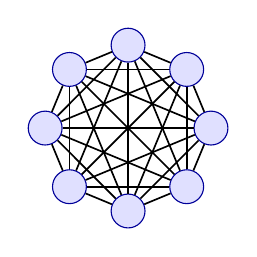
\begin{tikzpicture}[scale=0.78, every node/.style={circle,draw,fill=white,inner sep=1.3pt,minimum size=4.3mm,font=\scriptsize},
edge/.style={line width=0.6pt}, hl/.style={fill=blue!12,draw=blue!60!black}]
  \foreach \i/\ang in {1/90,2/45,3/0,4/315,5/270,6/225,7/180,8/135}{
    \node[hl] (n\i) at (\ang:1.35) {};
  }
  \foreach \i/\j in {1/2,1/3,1/4,1/5,1/6,1/7,1/8,2/3,2/4,2/5,2/6,2/7,2/8,3/4,3/5,3/6,3/7,3/8,4/5,4/6,4/7,4/8,5/6,5/7,5/8,6/7,6/8,7/8}{
    \draw[edge] (n\i)--(n\j);
  }
\end{tikzpicture}
\par\vspace{1mm}\scriptsize \textbf{(a) Global-best}
\end{minipage}
&
\begin{minipage}[t]{0.22\textwidth}\centering
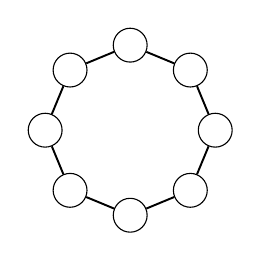
\begin{tikzpicture}[scale=0.8, every node/.style={circle,draw,fill=white,inner sep=1.3pt,minimum size=4.3mm,font=\scriptsize}, edge/.style={line width=0.7pt}]
  \foreach \i/\ang in {1/90,2/45,3/0,4/315,5/270,6/225,7/180,8/135}{
    \node (n\i) at (\ang:1.35) {};
  }
  \foreach \i/\j in {1/2,2/3,3/4,4/5,5/6,6/7,7/8,8/1}{\draw[edge] (n\i)--(n\j);}  
\end{tikzpicture}
\par\vspace{1mm}\scriptsize \textbf{(b) Ring}
\end{minipage}
&
\begin{minipage}[t]{0.22\textwidth}\centering
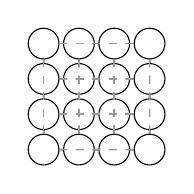
\begin{tikzpicture}[scale=0.66, every node/.style={circle,draw,fill=white,inner sep=1.0pt,minimum size=3.9mm,font=\scriptsize}, edge/.style={line width=0.6pt}, wrap/.style={line width=0.6pt,dashed,gray!80}]
  \foreach \r in {1,2,3,4}{
    \foreach \c in {1,2,3,4}{
      \pgfmathtruncatemacro{\id}{4*(\r-1)+\c}
      \node (n\id) at (0.68*\c, -0.68*\r) {};
    }
  }
  \foreach \r in {1,2,3,4}{
    \foreach \c in {1,2,3,4}{
      \pgfmathtruncatemacro{\cn}{mod(\c,4)+1}
      \pgfmathtruncatemacro{\a}{4*(\r-1)+\c}
      \pgfmathtruncatemacro{\b}{4*(\r-1)+\cn}
      \ifnum\c<4 \draw[edge] (n\a)--(n\b); \else \draw[wrap] (n\a)--(n\b); \fi
    }
  }
  \foreach \c in {1,2,3,4}{
    \foreach \r in {1,2,3,4}{
      \pgfmathtruncatemacro{\rn}{mod(\r,4)+1}
      \pgfmathtruncatemacro{\a}{4*(\r-1)+\c}
      \pgfmathtruncatemacro{\b}{4*(\rn-1)+\c}
      \ifnum\r<4 \draw[edge] (n\a)--(n\b); \else \draw[wrap] (n\a)--(n\b); \fi
    }
  }
\end{tikzpicture}
\par\vspace{1mm}\scriptsize \textbf{(c) Griglia von Neumann toroidale}
\end{minipage}
&
\begin{minipage}[t]{0.22\textwidth}\centering
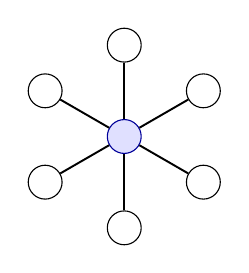
\begin{tikzpicture}[scale=0.8, every node/.style={circle,draw,fill=white,inner sep=1.3pt,minimum size=4.3mm,font=\scriptsize}, edge/.style={line width=0.7pt}, hub/.style={fill=blue!12,draw=blue!60!black}]
  \node[hub] (c) at (0,0) {};
  \foreach \i/\ang in {1/90,2/30,3/330,4/270,5/210,6/150}{
    \node (n\i) at (\ang:1.45) {};
    \draw[edge] (c)--(n\i);
  }
\end{tikzpicture}
\par\vspace{1mm}\scriptsize \textbf{(d) Wheel nell'API (hub-and-spoke)}
\end{minipage}
\\[1.8ex]
\begin{minipage}[t]{0.22\textwidth}\centering
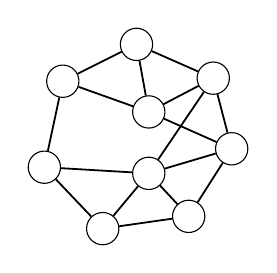
\begin{tikzpicture}[scale=0.78, every node/.style={circle,draw,fill=white,inner sep=1.1pt,minimum size=4.1mm,font=\scriptsize}, edge/.style={line width=0.65pt}]
  \foreach \i/\x/\y in {1/0/1.55,2/1.25/1.0,3/1.55/-0.15,4/0.85/-1.25,5/-0.55/-1.45,6/-1.5/-0.45,7/-1.2/0.95,8/0.2/0.45,9/0.2/-0.55}{
    \node (n\i) at (\x,\y) {};
  }
  \foreach \i/\j in {1/2,1/8,1/7,2/3,2/8,2/9,3/8,3/9,3/4,4/5,4/9,5/6,5/9,6/7,6/9,7/8}{\draw[edge] (n\i)--(n\j);}  
\end{tikzpicture}
\par\vspace{1mm}\scriptsize \textbf{(e) Random connessa, $k\approx4$}
\end{minipage}
&
\begin{minipage}[t]{0.22\textwidth}\centering
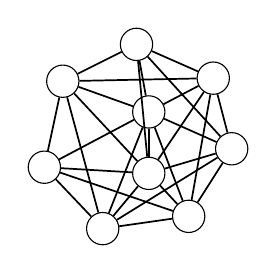
\begin{tikzpicture}[scale=0.78, every node/.style={circle,draw,fill=white,inner sep=1.1pt,minimum size=4.1mm,font=\scriptsize}, edge/.style={line width=0.62pt}]
  \foreach \i/\x/\y in {1/0/1.55,2/1.25/1.0,3/1.55/-0.15,4/0.85/-1.25,5/-0.55/-1.45,6/-1.5/-0.45,7/-1.2/0.95,8/0.2/0.45,9/0.2/-0.55}{
    \node (n\i) at (\x,\y) {};
  }
  \foreach \i/\j in {1/2,1/3,1/7,1/8,1/9,2/3,2/4,2/7,2/8,2/9,3/4,3/5,3/8,3/9,4/5,4/6,4/8,4/9,5/6,5/7,5/8,5/9,6/7,6/8,6/9,7/8,7/9,8/9}{\draw[edge] (n\i)--(n\j);}  
\end{tikzpicture}
\par\vspace{1mm}\scriptsize \textbf{(f) Random connessa, $k\approx8$}
\end{minipage}
&
\begin{minipage}[t]{0.22\textwidth}\centering
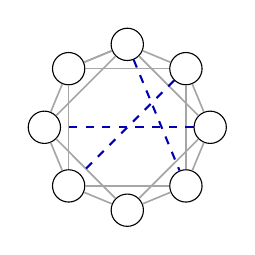
\begin{tikzpicture}[scale=0.78, every node/.style={circle,draw,fill=white,inner sep=1.1pt,minimum size=4.1mm,font=\scriptsize}, edge/.style={line width=0.6pt}, shortcut/.style={line width=0.75pt,blue!70!black,dashed}]
  \foreach \i/\ang in {1/90,2/45,3/0,4/315,5/270,6/225,7/180,8/135}{\node (n\i) at (\ang:1.35) {};}
  \foreach \i/\j in {1/2,2/3,3/4,4/5,5/6,6/7,7/8,8/1,1/8,1/3,2/4,3/5,4/6,5/7,6/8,7/1,8/2}{\draw[edge,gray!70] (n\i)--(n\j);} 
  \foreach \i/\j in {1/4,2/6,3/7}{\draw[shortcut] (n\i)--(n\j);}  
\end{tikzpicture}
\par\vspace{1mm}\scriptsize \textbf{(g) Small-world, $k=4$}
\end{minipage}
&
\begin{minipage}[t]{0.22\textwidth}\centering
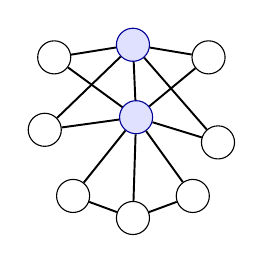
\begin{tikzpicture}[scale=0.8, every node/.style={circle,draw,fill=white,inner sep=1.1pt,minimum size=4.2mm,font=\scriptsize}, edge/.style={line width=0.7pt}, hub/.style={fill=blue!12,draw=blue!60!black}]
  \node[hub] (h1) at (0,1.2) {};
  \node[hub] (h2) at (0.05,0.05) {};
  \node (n3) at (-1.25,1.0) {};
  \node (n4) at (1.2,1.0) {};
  \node (n5) at (-1.4,-0.15) {};
  \node (n6) at (1.35,-0.35) {};
  \node (n7) at (-0.95,-1.2) {};
  \node (n8) at (0.95,-1.2) {};
  \node (n9) at (0,-1.55) {};
  \foreach \i/\j in {h1/h2,h1/n3,h1/n4,h1/n5,h1/n6,h2/n3,h2/n4,h2/n5,h2/n6,h2/n7,h2/n8,h2/n9,n7/n9,n8/n9}{\draw[edge] (\i)--(\j);}  
\end{tikzpicture}
\par\vspace{1mm}\scriptsize \textbf{(h) Scale-free, $k=4$}
\end{minipage}
\end{tabular}
\caption{Schemi TikZ delle otto topologie di comunicazione discusse nel manoscritto. I pannelli sono rappresentazioni qualitative della struttura del vicinato e non corrispondono alla dimensione reale dello sciame usata negli esperimenti. Per le topologie random, small-world e scale-free si mostrano realizzazioni esemplificative; la topologia \texttt{wheel} implementata nel codice coincide con una struttura hub-and-spoke, cio\`e una stella, e non con la wheel grafica standard dotata di anello periferico. Nella griglia von Neumann le linee tratteggiate indicano i collegamenti periodici della topologia toroidale.}
\label{fig:topology-schematics}
\end{figure*}

\subsection{Dinamica discreta e casualità per coordinata}
La PSO discreta di controllo sostituisce la propagazione locale con
\begin{equation}
\begin{aligned}
\bm v_i^{k+1}&=\mu_k\bm v_i^k+a_i^k(\bm p_i^k-\bm x_i^k)
+b_i^k(\bm s_i^k-\bm x_i^k),\\
\bm x_i^{k+1}&=\bm x_i^k+\bm v_i^{k+1}.
\end{aligned}\label{eq:controlled-discrete}
\end{equation}
Lo snapshot, il commit e la restituzione sono condivisi con il caso analitico. Nel controllo per coordinata si estrae una coppia $r_{1,ij}^k,r_{2,ij}^k$ per ogni $j$, applicando a ciascuna coordinata il corrispondente problema locale. Il disegno incrocia quindi due leggi di aggiornamento con due forme di casualità. I coefficienti scalari rendono comune alle coordinate la matrice locale di propagazione; nel codice esaminato la funzione analitica è comunque chiamata nel ciclo sulle coordinate. Le misure temporali riguardano questa implementazione.

\FloatBarrier
\section{Disegno sperimentale e criteri di analisi}\label{sec:exp}

\subsection{Piattaforma e sequenza delle campagne}
Le tre indagini principali sono organizzate come studi successivi, ciascuno con campione di selezione e campione di verifica. La prima determina la sensibilità al passo $h=\Delta t$; la seconda sceglie un framework CPSO mediante qualità e tempo di esecuzione; la terza trasferisce la configurazione congelata al confronto con dieci varianti PSO. I risultati delle figure di questo articolo derivano dal profilo \emph{pilot}, distinto dal profilo \emph{paper} predisposto nel codice e dalle campagne precedenti. L'inventario completo è riportato in Appendice~\ref{app:campaigns}.

I risultati sono stati ottenuti su MacBook Air con Apple M2, CPU a otto core (quattro performance e quattro efficiency) e memoria condivisa \citep{AppleM2Specs,AppleM2Design}. Il motore nativo C++20 adotta il propagatore analitico, un pool di thread, generatori di numeri casuali associati alle particelle e callback di valutazione. Le esecuzioni sincrone conservano lo snapshot a inizio generazione e il commit ordinato definiti nella Sezione~\ref{sec:model}; asincrono e isole realizzano semantiche di ricerca distinte. Popolazione, parametri dinamici e vincoli sono descritti in Appendice~\ref{app:campaigns}.

\subsection{Studio I: sensibilità al passo temporale}
Lo studio nativo comprende Sphere, Rastrigin, Rosenbrock, Ackley, Griewank e Salomon, a $D\in\{30,100\}$ e con $N=64$ particelle. Nel profilo pilot si valutano dodici passi su una griglia comprendente $0.38125$, $0.5$, $0.7$, $1$, $3.6$ e il riferimento $30$. Si eseguono tre budget indipendenti, $K\in\{15,63,127\}$ aggiornamenti, equivalenti a $B=N(K+1)\in\{1024,4096,8192\}$ FE. Ogni budget corrisponde a una run completa, con schedule di inerzia propria; non è un checkpoint di una traiettoria più lunga. Otto semi appaiati alimentano la selezione, dodici nuovi semi l'hold-out.

Con $f^*=0$ per queste funzioni, la metrica primaria è il log-residuo finale normalizzato rispetto al migliore valore iniziale:
\begin{equation}
 z(h;B)=\log_{10}\!\left[\operatorname{clip}_{[10^{-16},1]}
 \frac{\max\{f^{(B)}(h),0\}}{f^{(0)}}\right].\label{eq:dt-criterion}
\end{equation}
La metrica secondaria integra il medesimo log-residuo lungo le FE. Funzioni, dimensioni e budget hanno uguale peso nella sintesi. Il passo minimizzante viene scelto solo sui semi di selezione; i tre candidati migliori e $h=30$ sono poi confrontati, senza nuova ottimizzazione, sui semi dell'hold-out. Le differenze sono appaiate per seme e problema; gli intervalli derivano da bootstrap appaiato e i contrasti sono corretti secondo Holm.

\subsection{Studio II: selezione del framework multicore}
Si confrontano cinque organizzazioni: seriale, master--slave, particle-parallel, asincrono e isole. I backend sincroni differiscono per la distribuzione di propagazione e valutazioni; asincrono e isole modificano anche la dinamica effettiva degli aggiornamenti. Il fattore sociale comprende otto configurazioni (Global, ring, von Neumann, star, random R4/R8, small-world e scale-free). I worker assumono $p\in\{1,2,4,8\}$; il modello a isole usa quattro sottopopolazioni e, nel pilot, migrazione assente oppure ogni due o cinque aggiornamenti con grafo di migrazione ring o fully connected. Le combinazioni incompatibili con le dimensioni delle isole non sono generate.

La campagna pilot usa due funzioni di natura differente, Rastrigin e diffusione inversa, entrambe a $D=30,100$, $N=64$, $K=15$ e lavoro nativo controllato. Selezione e hold-out usano semi e sessioni distinti; il protocollo prevede riscaldamento e ordine randomizzato dei casi. Il criterio primario è la qualità finale della \emph{run completata}, misurata dal rapporto tra fitness finale e fitness iniziale; fra le configurazioni ammissibili per qualità, si minimizza il tempo geometrico wall-clock. Una perdita fino a $0.10$ unità logaritmiche rispetto alla migliore qualità osservata in selezione è ammissibile soltanto quando il limite superiore dell'intervallo bootstrap resta entro la soglia. Si congelano una scelta globale e scelte per obiettivo/dimensione, poi verificate su nuovi semi e sessioni.

Per i backend che riproducono la stessa traiettoria della seriale si distinguono accelerazione e strong scaling:
\begin{equation}
 A_a(p)=\frac{T_s}{T_{a,p}},\qquad
 S_a(p)=\frac{T_{a,1}}{T_{a,p}},\qquad
 E_a(p)=\frac{S_a(p)}p.\label{eq:speedup-efficiency}
\end{equation}
$T_s$ indica il tempo della seriale e $T_{a,p}$ il tempo del backend $a$ con $p$ worker. Le medie geometriche e gli intervalli bootstrap sono costruiti su rapporti appaiati. Per asincrono e isole il rapporto $T_s/T_{a,p}$ è denominato \emph{rapporto temporale} e non speedup di una traiettoria invariata. Il timer operativo è il wall-clock della chiamata completa, distinto dal cronometro del solver e dalle verifiche indipendenti dei valori obiettivo. Le curve di speedup ed efficienza si riferiscono ai soli backend sincroni.

\subsection{Studio III: confronto con la famiglia PSO}
La competizione nativa trasferisce il framework e il vicinato congelati dallo Studio II. Il CPSO così selezionato è il metodo principale; una sua esecuzione seriale con il medesimo vicinato serve da controllo e non partecipa al ranking, evitando di contare due volte la stessa famiglia. I concorrenti sono Classic gbest, Inertia gbest, Inertia lbest ring, Constriction, CLPSO, FIPS ring, SPSO-2011, SL-PSO, CSO e DMS-PSO, definiti in Appendice~\ref{app:baselines}. Le valutazioni effettive, inclusa la popolazione iniziale, sono pareggiate; ogni budget della scala richiede una run autonoma.

Nel pilot si considerano $D\in\{5,20,100\}$ e $B\in\{1024,4096,8192\}$ FE per sei funzioni native. I ranghi sono attribuiti entro problema a parità di budget, mantenendo eguale peso alle funzioni. Gli intervalli dei ranghi sono ottenuti ricampionando le funzioni; i confronti primari utilizzano differenze relative limitate e bootstrap per semi appaiati. I tempi rappresentano il costo delle implementazioni effettivamente eseguite: il CPSO utilizza C++ nativo, mentre le baseline utilizzano Python/NumPy con valutatori matematicamente corrispondenti. La verifica indipendente delle funzioni, inclusa la diffusione inversa con integrazione RK4, controlla la concordanza dei valori finali. Le figure costo--qualità collegano risultati di \emph{run completate} a budget diversi e non sono interpretate come curve al primo raggiungimento di un target.

Il controllo esterno BBOB comprende 24 funzioni, $D=5,20$, tre istanze del pilot e checkpoint a $64D$, $192D$ e $512D$ FE di una traiettoria programmata al budget massimo. Il riferimento CPSO viene eseguito serialmente per il vincolo dell'interfaccia callback corrente; la verifica BBOB riguarda quindi la qualità dell'algoritmo, non il guadagno multicore della configurazione asincrona. L'Observer COCO identifica i minimi e le soglie di target \citep{Hansen2021,Hansen2016Procedure}. L'ECDF conserva tutti gli insuccessi nel denominatore e usa 21 target, da $10^2$ a $10^{-8}$.

\subsection{Controlli statistici e studi complementari}
Le campagne precedenti comprendono la replica BBOB a nuovo seme, il confronto nello stesso motore fra propagatore analitico e discreto, l'ablazione della casualità scalare/per coordinata e una diagnostica geometrica a $D=1000$. Restano disponibili come risultati complementari nelle Appendici~\ref{app:external-ranks} e~\ref{app:controlled-results}, senza sostituire il confronto principale con CPSO parallelo. Per gli effetti appaiati controllati si mantiene la metrica
\begin{equation}
 d_{L,R}=\frac{g_L-g_R}{\max(g_L+g_R,10^{-16})},\qquad
 g=\max(f-f^*,0),\label{eq:relative-effect}
\end{equation}
con valori negativi favorevoli a $L$. Le famiglie inferenziali e l'unità di ricampionamento rimangono quelle dichiarate nelle rispettive campagne \citep{Demsar2006,Garcia2010}.

L'analisi temporale a costo sintetico controllato mantiene inoltre il modello empirico a coefficienti non negativi
\begin{equation}
 \widehat T_{a,p}=aB+b\frac{B\widehat\tau_f}{p}+cp,
 \quad a,b,c\ge0,\label{eq:overhead-model}
\end{equation}
con \emph{regret} decisionale $R=T_{a,\widehat p}/\min_p T_{a,p}-1$ (Appendice~\ref{app:parallel-results}); questo studio quantifica separatamente l'effetto della granularità del lavoro e non determina la scelta del framework nella campagna pilot.

\FloatBarrier


\paragraph{Disponibilit\`a del codice e tracciabilit\`a.}
L'implementazione e gli script delle campagne sono disponibili nel repository \href{https://github.com/GiovanniIacuzzo/Parallel-Continuous-Particle-Swarm-Optimization}{Parallel-Continuous-Particle-Swarm-Optimization} dell'Autore. Le configurazioni sorgente, i manifest e i dati prodotti dalle singole campagne costituiscono la base per la futura sezione sperimentale; l'esistenza di un protocollo nel codice non ne implica l'avvenuto completamento.

\clearpage
\bibliographystyle{unsrtnat}
\bibliography{references}
\clearpage\onecolumn\appendix
\numberwithin{figure}{section}
\numberwithin{table}{section}
\numberwithin{equation}{section}
\setlength{\parskip}{0pt}
\section{Propagatore analitico, grafi e dettagli dei backend}
\label{app:dynamics}


\subsection{Soluzione analitica nella notazione del PDF}
Nella notazione originale, le radici dell'Eq.~(13) sono
\begin{equation}
 \lambda_1^k=-\omega_k\left[\zeta_k+\sqrt{\zeta_k^2-1}\right],\qquad
 \lambda_2^k=-\omega_k\left[\zeta_k-\sqrt{\zeta_k^2-1}\right].
 \label{eq:or-roots}
\end{equation}
Per $\lambda_1^k\ne\lambda_2^k$, le Eqq.~(14)--(15) del PDF riportano
\begin{equation}
 p_{[(k-1)dt,kdt]}(t)=c_1^k\exp(\lambda_1^k t)
 +c_2^k\exp(\lambda_2^k t)+\frac{f_k}{\omega_k^2},
 \label{eq:or-distinct-solution}
\end{equation}
\begin{equation}
 c_1^k=\frac{\left(p_k-\dfrac{f_k}{\omega_k^2}\right)\lambda_2^k-\dot p_k}
 {(\lambda_2^k-\lambda_1^k)\exp(\lambda_1^k kdt)},\qquad
 c_2^k=\frac{\dot p_k-\left(p_k-\dfrac{f_k}{\omega_k^2}\right)\lambda_1^k}
 {(\lambda_2^k-\lambda_1^k)\exp(\lambda_2^k kdt)}.
 \label{eq:or-distinct-coefficients}
\end{equation}
Per $\lambda_1^k=\lambda_2^k=\overline\lambda^k$, le Eqq.~(16)--(18) originali sono
\begin{equation}
 p_{[(k-1)dt,kdt]}(t)=(c_1^k+c_2^k t)\exp(\overline\lambda^k t)
 +\frac{f_k}{\omega_k^2},\label{eq:or-critical-solution}
\end{equation}
\begin{equation}
 c_1^k=\left[\left(p_k-\frac{f_k}{\omega_k^2}\right)(1+\overline\lambda^k kdt)
 -\dot p_k kdt\right]\exp(-\overline\lambda^k kdt),\label{eq:or-critical-c1}
\end{equation}
\begin{equation}
 c_2^k=\dot p_k-\overline\lambda^k\left(p_k-\frac{f_k}{\omega_k^2}\right).
 \label{eq:or-critical-c2-printed}
\end{equation}
Queste espressioni mantengono la forma stampata nel PDF, compreso l'indice dell'intervallo nelle Eqq.~(14) e~(16). L'Eq.~(10) della stessa fonte usa invece $[kdt,(k+1)dt]$. Inoltre, per una scrittura in tempo assoluto, imporre $p(kdt)=p_k$ e $\dot p(kdt)=\dot p_k$ richiede nel secondo coefficiente critico il fattore $\exp(-\overline\lambda^k kdt)$, assente nell'Eq.~(18) stampata. La trascrizione dell'Eq.~\eqref{eq:or-critical-c2-printed} conserva tale formula; la valutazione numerica sottostante usa il tempo locale $\tau=t-kdt$, con condizioni iniziali a $\tau=0$. Questa distinzione evita di assimilare una correzione matematica alla riproduzione testuale della fonte.

Nella fonte $\omega$ è la pulsazione non smorzata e $\zeta$ il rapporto di smorzamento. Con $\alpha=\zeta\omega$, la pulsazione smorzata è $\nu=\omega\sqrt{1-\zeta^2}$ quando $\zeta<1$. Il testo seguente usa $q=\omega_k^2$ e $\alpha=\zeta_k\omega_k$ per le formule numeriche, mantenendo distinta $\nu$ da $\omega_k$.

\subsection{Valutazione numerica in tempo locale}
Si consideri una singola coordinata della dinamica~\eqref{eq:cpso-model}. Posto $a=c_c r_1$, $b=c_s r_2$, $q=a+b$, $\alpha=(1-\mu_k)/2$ e $F=ap+bs$, il problema locale \`e $x''+2\alpha x'+qx=F$. Per $q>0$ si definiscono $x_{\rm eq}=F/q$ e $y=x-x_{\rm eq}$; allora
\begin{equation}
 y''+2\alpha y'+qy=0,\quad y(0)=x^k-x_{\rm eq},\quad y'(0)=v^k.
 \label{eq:app-frozen}
\end{equation}
Con $h=\Delta t$ e $\Delta=\alpha^2-q$, il propagatore C++ distingue i tre casi seguenti.

\paragraph{Sottosmorzamento ($\Delta<0$).}
Definiti $\nu=\sqrt{-\Delta}$, $C=(v^k+\alpha y_0)/\nu$, $G=y_0\cos(\nu h)+C\sin(\nu h)$, si ha
\begin{equation}
 y(h)=e^{-\alpha h}G,\quad
 v(h)=e^{-\alpha h}\big[-\nu y_0\sin(\nu h)+\nu C\cos(\nu h)-\alpha G\big].
\end{equation}

\paragraph{Sovrasmorzamento ($\Delta>0$).}
Siano $\lambda_{1,2}=-\alpha\pm\sqrt{\Delta}$ e
\begin{equation}
 C_1=\frac{v^k-\lambda_2y_0}{\lambda_1-\lambda_2},\qquad
 C_2=\frac{\lambda_1y_0-v^k}{\lambda_1-\lambda_2}.
\end{equation}
Allora $y(h)=C_1e^{\lambda_1h}+C_2e^{\lambda_2h}$ e
$v(h)=\lambda_1C_1e^{\lambda_1h}+\lambda_2C_2e^{\lambda_2h}$.

\paragraph{Smorzamento critico ($\Delta=0$).}
Posto $C_2=v^k+\alpha y_0$,
\begin{equation}
 y(h)=e^{-\alpha h}(y_0+C_2h),\qquad
 v(h)=e^{-\alpha h}(v^k-\alpha C_2h).
\end{equation}
La posizione finale \`e $x^{k+1}=x_{\rm eq}+y(h)$; le formule restituiscono contemporaneamente la velocit\`a $v^{k+1}=v(h)$. L'implementazione definisce il caso numericamente critico mediante $|\Delta|\le 64\epsilon_{\rm mach}\max\{1,\alpha^2,q\}$. Il criterio \`e una tolleranza di floating point, non un quarto regime fisico.

Se $q=0$, i coefficienti non negativi implicano $a=b=F=0$. La formula generale del propagatore, chiamato con equilibrio pari a zero, risolve il sistema omogeneo con una radice nulla e una radice $-2\alpha$; per $\alpha>0$ coincide con
\begin{equation}
 v(h)=v^k e^{-2\alpha h},\qquad
 x(h)=x^k+\frac{1-e^{-2\alpha h}}{2\alpha}v^k,
\end{equation}
mentre per $\alpha=0$ si ha $x(h)=x^k+hv^k$, $v(h)=v^k$. La scelta $q=0$ ha probabilit\`a nulla sotto coefficienti casuali uniformi non degeneri, ma viene comunque gestita in modo consistente.

L'inerzia \`e calcolata con il contatore $k$ dei $K$ aggiornamenti programmati:
\begin{equation}
\mu_k=\mu_{\max}-\frac{k}{K-1}(\mu_{\max}-\mu_{\min}),
\quad k=0,\dots,K-1\quad (K>1),
\label{eq:code-inertia-schedule}
\end{equation}
e $\mu_0=\mu_{\max}$ se $K=1$. L'estrazione $r_1,r_2$ avviene una volta per particella e intervallo ed \`e condivisa fra coordinate. La mappa di confinamento applica
\begin{equation}
(x_j,v_j)\mapsto
\begin{cases}
(\ell_j,-ev_j),&x_j<\ell_j,\ v_j<0,\\
(\ell_j,v_j),&x_j<\ell_j,\ v_j\ge0,\\
(u_j,-ev_j),&x_j>u_j,\ v_j>0,\\
(u_j,v_j),&x_j>u_j,\ v_j\le0,\\
(x_j,v_j),&\text{altrimenti};
\end{cases}
\end{equation}
la valutazione segue la correzione. La propagazione analitica locale e il clipping costituiscono due trasformazioni algoritmiche distinte.

\subsection{Costruzione esatta dei vicinati}
Le reti non orientate sono statiche all'interno di una run; la lista dei vicini include sempre il nodo stesso, viene ordinata e non contiene duplicati. Per il caso global-best il leader \`e l'incumbent globale, con conservazione dell'indice in caso di parit\`a; per gli altri grafi gli ex aequo selezionano l'indice minimo. La Tabella~\ref{tab:app-graphs} identifica le otto configurazioni usate dai runner di scaling e topologia.

\begin{table}[H]
\centering\small
\caption{Le otto configurazioni di vicinato corrispondenti a sette famiglie di grafo. I gradi delle reti random sono parametri di campionamento, non gradi realizzati imposti a ogni vertice.}
\label{tab:app-graphs}
\begin{tabularx}{\textwidth}{@{}p{3.0cm}X@{}}
\toprule
Configurazione & Costruzione nel codice \\
\midrule
Global-best & Leader scelto tra i personal best di tutte le particelle.\\
Ring & Due vicini periodici ($i-1,i+1$), pi\`u self.\\
Von Neumann & Griglia toroidale con quattro adiacenze ortogonali; per $N=64$ la forma \`e $8\times8$.\\
Star (stella) & Stella con un hub e archi hub--periferia; hub assegnato a un indice casuale. Nessun arco fra periferici.\\
Random $k=4$ & Campionamento Bernoulli con $p=4/(N-1)$ e connessione delle componenti residue con ponti.\\
Random $k=8$ & Stessa costruzione con $p=8/(N-1)$; \`e la seconda impostazione di una stessa famiglia.\\
Small-world $k=4$ & Anello iniziale di grado quattro, rewiring per arco con probabilit\`a $0.15$.\\
Scale-free $k=4$ & Crescita per attaccamento preferenziale con $m=k/2=2$ archi per nuovo nodo; clique iniziale di tre nodi e permutazione finale degli indici.\\
\bottomrule
\end{tabularx}
\end{table}

L'algoritmo che collega le componenti del grafo Bernoulli mediante ponti \`e differente dalla generazione condizionata di $G(N,p)$ a connettivit\`a imposta. Le permutazioni di hub e nodi scale-free servono a non associare sistematicamente i ruoli strutturali agli indici che determinano gli stream casuali delle particelle.


\subsection{Contabilizzazione delle generazioni}
Una storia sincrona contiene un best iniziale e uno per generazione, agli ascissi $N,2N,\ldots,(K+1)N$. Gli esperimenti recenti confrontano storia e posizione mediante hash a parità di seme e lavoro, controllando separatamente il budget FE. Il pool C++ rimane attivo durante la run; i task acquisiscono dinamicamente indici da un contatore atomico e il thread chiamante attende la fine del lotto. Snapshot e commit avvengono ai confini delle generazioni.

\subsection{Lettura spettrale del passo}
Per il problema a equilibrio congelato, lo stato $(y,v)$ evolve mediante $e^{hL}$ con
\begin{equation}
 L=\begin{pmatrix}0&1\\-q&-2\alpha\end{pmatrix},\qquad
 \lambda_\pm=-\alpha\pm\sqrt{\alpha^2-q}.
\end{equation}
Nel regime sottosmorzato, il raggio spettrale del flusso è $e^{-\alpha h}$ e la fase è $h\sqrt{q-\alpha^2}$. Con $c_c=c_s=2.05$ e due uniformi indipendenti, $q$ varia fra 0 e 4.1, mentre $\alpha\in[0.05,0.30]$. Il regime sottosmorzato occupa quindi quasi tutto il dominio dei coefficienti. La Tabella~\ref{tab:local-envelope} riporta valori analitici dell'inviluppo.
\begin{table}[H]\centering\small
\caption{Fattore d'inviluppo $e^{-\alpha h}$ del flusso sottosmorzato a coefficienti congelati. I valori sono calcolati dalla formula, indipendentemente dalle run di ottimizzazione.}\label{tab:local-envelope}
\begin{tabular}{@{}rrrrr@{}}\toprule
$\mu$ & $\alpha$ & $h=0.38125$ & $h=1$ & $h=30$\\\midrule
0.4 & 0.300 & 0.8919 & 0.7408 & 0.0001234\\
0.65 & 0.175 & 0.9355 & 0.8395 & 0.005248\\
0.9 & 0.050 & 0.9811 & 0.9512 & 0.223130\\\bottomrule
\end{tabular}\end{table}

La PSO discreta a passo unitario, con lo stesso equilibrio congelato, ha matrice
\begin{equation}
 M(q,\mu)=\begin{pmatrix}1-q&\mu\\-q&\mu\end{pmatrix},\qquad
 \det M=\mu,\quad \operatorname{tr}M=1-q+\mu.
\end{equation}
Per $0<\mu<1$ le condizioni di Schur sono $0<q<2(1+\mu)$. In particolare alcuni valori possibili di $q$ oltrepassano tale soglia. Il fattore di costrizione $\chi\simeq0.7298$ sostituisce la matrice con $M(\chi q,\chi)$ e cambia quindi una diversa legge di aggiornamento. Una corrispondenza basata solo sull'inviluppo uguaglierebbe $e^{-\alpha h}$ a $\sqrt\chi$ nel regime di autovalori complessi: essa non uguaglia fase e attrattori. Queste relazioni descrivono la stabilità locale a coefficienti congelati; leader e coefficienti della ricerca cambiano dopo ciascuna FE.

\subsection{Obiettivi interni e diffusione inversa}
Le sei funzioni di screening sono le formulazioni standard non traslate: Sphere $\sum_jx_j^2$; Rastrigin $10D+\sum_j[x_j^2-10\cos(2\pi x_j)]$; Rosenbrock $\sum_{j=1}^{D-1}[100(x_{j+1}-x_j^2)^2+(1-x_j)^2]$; Ackley con parametri $20,0.2,2\pi$; Griewank $1+\sum_jx_j^2/4000-\prod_j\cos(x_j/\sqrt j)$; Salomon $1-\cos(2\pi\|x\|)+0.1\|x\|$. Gli ottimi sono nell'origine, tranne Rosenbrock in $\bm1$, tutti con minimo zero. I box di default del runner sono rispettivamente $[-100,100]$, $[-5.12,5.12]$, $[-5,10]$, $[-32.768,32.768]$, $[-600,600]$ e $[-100,100]$ per coordinata.

L'obiettivo denominato diffusione inversa è un problema sintetico deterministico di identificazione della sorgente. Con $D$ variabili, il vettore di verità è $\theta_j^\dagger=0.4\sin(2\pi j/(D+1))$, $j=1,\ldots,D$. Si integra lo stato differenza $u(0)=0$:
\begin{equation}
 \dot u_j=-\lambda_ju_j+0.2(u_{j-1}-2u_j+u_{j+1})
 +[1+0.2\sin(2\pi t)]\,[\tanh\theta_j-\tanh\theta_j^\dagger],
\end{equation}
con $u_0=u_1$, $u_{D+1}=u_D$ e $\lambda_j=1.1+0.02((j-1)\bmod11)$. Il tempo finale è $2$. La differenza spaziale usa il coefficiente scritto, senza un fattore $\Delta x^{-2}$: il benchmark è il sistema semidiscreto così definito. Si usa RK4 e si osserva lo stato a quattro tempi equispaziati. La funzione obiettivo è
\begin{equation}
 f(\theta)=\frac{1}{4D}\sum_{m=1}^4\sum_{j=1}^D u_j(m/2)^2
 +\frac{10^{-3}}D\sum_{j=1}^D(\theta_j-\theta_j^\dagger)^2.
\end{equation}
Il minimo noto è zero in $\theta^\dagger$. Nello studio topologico il numero di passi RK4 è 256 e il box del driver è $[-2,2]^D$. Il lavoro RK4 viene mantenuto identico fra backend entro ciascuna cella.

\FloatBarrier
\section{Formulazioni e configurazioni delle baseline PSO}
\label{app:baselines}

Le baseline sono algoritmi PSO discreti in spazio decisionale continuo. Le formule seguenti specificano le configurazioni dello Studio III, inclusi gli adattamenti di popolazione, dominio e budget.

\subsection{Parametri e adattamenti comuni}

Nello Studio III la popolazione è fissata a $N=100$. Le campagne a FE fissate assegnano lo stesso budget per problema e metodo. La campagna temporale assegna la stessa durata. Le misure sono appaiate per blocco sperimentale. La velocità iniziale è in generale campionata in $[-0.1w_j,0.1w_j]$, dove $w_j=u_j-\ell_j$; SL-PSO e Competitive Swarm Optimizer iniziano con velocità nulla, mentre SPSO-2011 usa la propria inizializzazione nel box normalizzato.

\begin{table}[H]
\centering
\caption{Configurazioni delle baseline dichiarate nel protocollo. $V_{\max}$ è espresso come frazione della larghezza del dominio.}
\label{tab:app-baseline-config}
\small
\begin{tabularx}{\textwidth}{@{}lXllX@{}}
\toprule
Metodo & Parametri/controlli principali & $V_{\max}$ & $v^0$ & Nota di adattamento \\
\midrule
Classic global-best & $c_1=c_2=2$, $w=1$ & $0.2w_j$ & $U[-0.1w_j,0.1w_j]$ & PSO gbest senza inerzia variabile; clipping e restituzione comuni. \\
Inertia global-best & $c_1=c_2=2.05$, $w:0.9\to0.4$ & $0.2w_j$ & $U[-0.1w_j,0.1w_j]$ & Schedule lineare associata allo studio empirico di Shi--Eberhart 1999. \\
Constriction global-best & $c_1=c_2=2.05$, $\chi$ di Clerc--Kennedy & Nessuno & $U[-0.1w_j,0.1w_j]$ & Nessun limite di velocità nella configurazione corrente. \\
Inertia local-best ring & $c_1=c_2=2.05$, $w:0.9\to0.4$, raggio 1 & $0.2w_j$ & $U[-0.1w_j,0.1w_j]$ & Snapshot sincrono con vicinato periodico. \\
CLPSO & $c=1.49445$, $w:0.9\to0.4$, refresh 7 & $0.2w_j$ & $U[-0.1w_j,0.1w_j]$ & Esemplari per coordinata e probabilità di apprendimento dipendente dall'indice. \\
SL-PSO & $M=100$, $\alpha=0.5$, $\beta=0.01$ & Nessuno & $0$ & Formula di apprendimento conforme; popolazione fissata a 100 nello Studio III. \\
SPSO-2011 & $K_{\mathrm{informant}}=3$, $c=0.5+\ln2$, $\omega=(2\ln2)^{-1}$ & Nessuno & Box normalizzato & Direzioni uniformi e raggio uniforme; regola di confinamento SPSO-2011. \\
FIPS ring & $\phi=4.1$, due vicini, $\chi$ di costrizione & Nessuno & $U[-0.1w_j,0.1w_j]$ & Coefficienti casuali per coordinata, ring escluso il self. \\
Competitive Swarm Optimizer & $\varphi=0.1$, matching casuale & Nessuno & $0$ & Soli perdenti aggiornati; $N/2$ FE per generazione se $N$ è pari. \\
DMS-PSO & $c_1=c_2=2$, $w:0.9\to0.2$, gruppo obiettivo 3, regroup 5 & $0.2w_j$ & $U[-0.1w_j,0.1w_j]$ & Variante base senza ricerca locale quasi-Newton. \\
\bottomrule
\end{tabularx}
\end{table}

Per i metodi con limite di velocità, $V_{\max}=0.2(u_j-\ell_j)$ per coordinata. La mappa clamp--restitution è comune per i metodi che non prescrivono una regola di confinamento propria; SPSO-2011 mantiene il proprio clipping e inversione della componente uscente. Nelle iterazioni sincrone gli attrattori restano fissati fino al completamento del lotto.

\subsection{Fattore di costrizione}

La PSO con fattore di costrizione usa
\begin{equation}
 \chi=\frac{2}{\left|2-\varphi-\sqrt{\varphi^2-4\varphi}\right|}
 =\frac{2}{\varphi-2+\sqrt{\varphi^2-4\varphi}},
 \quad \varphi=c_1+c_2>4.
 \label{eq:app-clerc}
\end{equation}
Per $c_1=c_2=2.05$, $\varphi=4.1$ e $\chi\simeq0.7298$. Le due espressioni sono equivalenti per $\varphi>4$.

\subsection{Inerzia e CLPSO}

La baseline con inerzia utilizza $w_t$ decrescente linearmente da $0.9$ a $0.4$, con coefficienti $c_1=c_2=2.05$. L'introduzione del peso d'inerzia è associata a Shi ed Eberhart 1998, mentre lo studio empirico da cui si riprende la schedule lineare è citato separatamente come Shi ed Eberhart 1999 \citep{ShiEberhart1998,ShiEberhart1999}. Per CLPSO, la probabilità di apprendimento è
\begin{equation}
 P_{c,i}=0.05+0.45\frac{\exp\left(10i/(N-1)\right)-1}{\exp(10)-1},
 \qquad i=0,\ldots,N-1,
 \label{eq:app-clpso-pc}
\end{equation}
con esemplari selezionati per coordinata, $c=1.49445$ e refresh gap pari a sette generazioni. La baseline usa lo snapshot congelato e il limite di velocità $0.2$ volte la larghezza del dominio.

\subsection{SL-PSO e dimensione della popolazione}

SL-PSO ordina la popolazione dal peggiore al migliore. Ogni particella può apprendere da dimostratori che hanno un valore obiettivo inferiore al suo. La legge di probabilità di apprendimento \citep{ChengJin2015SLPSO} è espressa mediante il rango $r=0,\ldots,N-2$:
\begin{equation}
 \gamma=\beta\frac{D}{M},\qquad
 P_r=\left(1-\frac{r}{N}\right)^\eta,
 \qquad \eta=\alpha\log\!\left(\max\left\{1,\left\lceil\frac{D}{M}\right\rceil\right\}\right),
 \label{eq:app-slpso-impl}
\end{equation}
con $M=100$, $\alpha=0.5$, $\beta=0.01$. Nella notazione originale, che usa il rango one-based $i=1,\ldots,m-1$, la probabilità è $P_i^L=(1-(i-1)/m)^{\alpha\log\lceil D/M\rceil}$; ponendo $r=i-1$ e $N=m$ si ottiene la forma precedente. Per $D,M>0$ si ha $\lceil D/M\rceil\geq1$. Se l'apprendimento viene attivato, per ogni coordinata è selezionato un dimostratore migliore e lo spostamento è
\begin{equation}
 \Delta x_{i,j}^{t+1}=r_1v_{i,j}^t
 +r_2(x_{k(i,j),j}^t-x_{i,j}^t)
 +r_3\gamma(\bar x_j^t-x_{i,j}^t),
 \label{eq:app-slpso-update}
\end{equation}
con $r_1,r_2,r_3\sim U(0,1)$ e un dimostratore selezionato indipendentemente per coordinata fra le particelle migliori. La popolazione comune di $N=100$ particelle sostituisce qui la regola dimensionale $m=M+\lfloor D/10\rfloor$ con $M=100$.
\subsection{SPSO-2011}

La baseline SPSO-2011 costruisce un grafo diretto casuale di informant con $K=3$ informant più il self. Sia $p_i$ il personal best e $l_i$ il miglior personal best nell'insieme di informant. Il centro di gravità è
\begin{equation}
 G_i=x_i+c\frac{p_i+l_i-2x_i}{3},
 \quad c=\frac12+\ln2,
 \label{eq:app-spso-center}
\end{equation}
con il centro a due punti $G_i=x_i+c(p_i-x_i)/2$ nel caso $p_i=l_i$. Il campione $x_i'$ è estratto dall'ipersfera centrata in $G_i$ e di raggio $\|G_i-x_i\|$, con direzione uniforme e raggio uniforme. L'aggiornamento è
\begin{equation}
 v_i^{t+1}=\omega v_i^t+x_i'-x_i^t,
 \qquad x_i^{t+1}=x_i^t+v_i^{t+1},
 \qquad \omega=(2\ln2)^{-1}.
 \label{eq:app-spso-update}
\end{equation}
Le coordinate sono normalizzate nel box unitario per la costruzione geometrica e riportate al dominio originale. Il grafo viene rigenerato dopo una generazione senza miglioramento del migliore punto globale. Si applica la regola di confinamento SPSO-2011.

\subsection{FIPS}

La baseline FIPS usa il ring periodico a due vicini, escludendo la particella centrale. L'aggiornamento è
\begin{equation}
 v_i^{t+1}=\chi v_i^t+\frac{\chi}{|\mathcal N_i|}
 \sum_{j\in\mathcal N_i}R_{ij}\odot(p_j-x_i^t),
 \quad R_{ij,k}\sim U(0,\phi),\quad \phi=4.1,
 \label{eq:app-fips}
\end{equation}
con $\chi=2/(\phi-2+\sqrt{\phi^2-4\phi})$. I pesi casuali sono campionati per coordinata e l'anello di grado due resta fisso per tutta l'esecuzione.

\subsection{Competitive Swarm Optimizer e DMS-PSO}

Nel Competitive Swarm Optimizer (CSO), le particelle vengono accoppiate casualmente. Il vincitore resta invariato; il perdente aggiorna
\begin{equation}
\begin{aligned}
 v_l^{t+1}&=r_1\odot v_l^t+r_2\odot(x_w^t-x_l^t)
 +\varphi_{\mathrm{CSO}}r_3\odot(\bar x^t-x_l^t),\\
 x_l^{t+1}&=x_l^t+v_l^{t+1},\qquad \varphi_{\mathrm{CSO}}=0.1,
\end{aligned}
\label{eq:app-cso}
\end{equation}
con coefficienti casuali vettoriali. Soltanto i perdenti vengono rivalutati e una generazione completa consuma $N/2$ FE se $N$ è pari.

La baseline DMS-PSO usa sottosciami di dimensione obiettivo tre, riorganizzati casualmente ogni cinque generazioni. L'aggiornamento è
\begin{equation}
\begin{aligned}
 v_i^{t+1}&=\omega_t v_i^t+2r_1\odot(p_i-x_i^t)
 +2r_2\odot(l_i-x_i^t),\\
 x_i^{t+1}&=x_i^t+v_i^{t+1},
\end{aligned}
\label{eq:app-dms}
\end{equation}
con inerzia lineare da $0.9$ a $0.2$. Si usa la variante base. Le particelle rimaste dopo la partizione sono assegnate all'ultimo sottosciame.


\FloatBarrier
\section{Casualit\`a scalare e sottospazi invarianti del propagatore non vincolato}
\label{app:scalar-randomness}

Una scelta implementativa rilevante \`e l'uso di due numeri casuali scalari per particella e aggiornamento, riutilizzati in tutte le coordinate. Questa convenzione coincide con il codice in \texttt{optimizer\_internal.hpp} e nel backend asincrono. La sua conseguenza geometrica riguarda il tratto di dinamica privo di correzioni al dominio e va distinta da un'asserzione di convergenza.

\begin{proposition}[Invarianza dello span per la dinamica non corretta]
Siano $\bm x_i^0,\bm v_i^0\in\R^D$, $i=1,\ldots,N$, e
\begin{equation}
\mathcal S_0=\operatorname{span}\{\bm x_1^0,\ldots,\bm x_N^0,
\bm v_1^0,\ldots,\bm v_N^0\}.
\end{equation}
Supponiamo che i coefficienti del propagatore locale siano scalari comuni alle coordinate di una particella; che i leader sociali e i migliori personali siano posizioni gi\`a generate; e che nessuna correzione al dominio o operazione esterna introduca nuovi vettori. Allora, per ogni particella e ogni aggiornamento, posizioni, velocit\`a, migliori personali e leader appartengono a $\mathcal S_0$, con
$\dim\mathcal S_0\le\min\{D,2N\}$.
\end{proposition}

\begin{proof}
La tesi vale all'inizializzazione. Supponiamo valga al passo $k$. Il migliore personale e il leader sociale sono elementi di $\mathcal S_0$ per ipotesi induttiva. Se $q=a+b>0$, l'equilibrio $\bm x_{\rm eq}=(a\bm p+b\bm s)/q$ appartiene a $\mathcal S_0$. La soluzione di un sistema lineare scalare identico lungo ciascuna coordinata \`e una combinazione lineare di $\bm x^k$, $\bm v^k$ e $\bm x_{\rm eq}$, con gli stessi coefficienti scalari in tutte le coordinate; quindi $\bm x^{k+1},\bm v^{k+1}\in\mathcal S_0$. Per $q=0$ la soluzione \`e combinazione dei soli $\bm x^k$ e $\bm v^k$. La selezione di un nuovo best da posizioni generate preserva lo span. L'induzione conclude la prova e la stima dimensionale segue dal numero dei generatori.
\end{proof}

\paragraph{Limiti della proposizione.}
Il clipping componente per componente non \`e in generale una trasformazione lineare comune a tutte le coordinate, e pu\`o rompere l'invarianza. Anche l'introduzione di un immigrato proveniente da un'altra isola pu\`o ampliare lo span locale. Pertanto non \`e corretto interpretare $\dim\mathcal S_0\le2N$ come una restrizione assoluta dell'implementazione con vincoli attivi.

\paragraph{Interpretazione rispetto ai problemi studiati.}
Per $N=64$ il limite superiore $2N=128$ non impone uno span proprio nelle dimensioni interne $D=30,100$. Per il confronto esterno con $N=40$, il valore $2N=80$ \`e invece inferiore alle dimensioni di CEC 2013 LSGO e ad alcune dimensioni del protocollo esteso BBOB-LargeScale. Questa osservazione segnala un possibile meccanismo geometrico da misurare, non una prova di scarsa prestazione: il rango effettivo dipende anche da inizializzazione, box, traiettorie e correzioni. Nelle isole omogenee di dimensione locale $n$, il corrispondente limite \`e $2n$ prima di migrazione e correzioni. Un'eventuale versione con coefficienti casuali indipendenti per coordinata rappresenterebbe un algoritmo distinto e non viene confusa con la CPSO attualmente confrontata.

\FloatBarrier
\section{Campagne completate e tracciabilità}\label{app:campaigns}
La Tabella~\ref{tab:campaigns} distingue gli esperimenti storici dagli approfondimenti disponibili con la revisione. I conteggi si riferiscono a run, record o lotti secondo l'unità indicata. Le configurazioni estese presenti nel software costituiscono proposte di ulteriori esperimenti e sono escluse dai risultati di questo articolo.
\begin{table}[H]\centering\small
\caption{Inventario delle evidenze usate nel manoscritto.}\label{tab:campaigns}
\begin{tabularx}{\textwidth}{@{}p{3.3cm}Xr@{}}\toprule
Esperimento & Disegno completato & Quantità\\\midrule
Screening del passo & 6 funzioni, 2 dimensioni, 5 passi, 5 semi, $K=30$ & 300 run\\
Validazione del passo & 12 celle, 4 passi, 30 nuovi semi, $K=30$ & 1\,440 run\\
Topologie interne & 4 celle, 8 grafi, 24 semi, 3 ripetizioni, 4 worker count & 9\,216 run\\
BBOB iniziale & 24 funzioni, 2 dimensioni, 5 istanze, 12 metodi & 2\,880 run\\
Calibrazione BBOB & 24 funzioni, 2 dimensioni, 3 istanze, 4 passi & 576 run\\
Validazione BBOB & 24 funzioni, 2 dimensioni, 5 istanze, 13 etichette & 3\,120 record\\
CEC a budget ridotto & 15 funzioni, 5 semi, 12 metodi & 900 run\\
Replica BBOB $D=5$ & 24 funzioni, 5 istanze, 11 metodi, nuovo seme & 1\,320 run\\
Ablazione controllata & 4 funzioni, 2 dimensioni, 3 istanze, 65 metodi & 1\,560 run\\
Costo e parallelismo & 3 sessioni, 4 costi, 2 dinamiche, 2 ripetizioni, 12 modalità; 8 semi per lotto & 576 lotti\\
Diagnostica affine & 3 dimensioni, 3 semi, 16 configurazioni & 144 run\\
\bottomrule\end{tabularx}\end{table}

\subsection{Parametri condivisi ed eccezioni}
Il nucleo usa $c_c=c_s=2.05$, $\mu_{\max}=0.9$, $\mu_{\min}=0.4$, velocità iniziale uniforme in $[-0.1w_j,0.1w_j]$ e restituzione $e=0.5$. La popolazione è $N=64$. Il passo delle topologie e degli approfondimenti temporali e geometrici è $1$. Il fattoriale varia il passo analitico; la comparazione esterna trasferisce quello selezionato nel proprio disegno. Le schedule d'inerzia dipendono dal budget programmato: un checkpoint intermedio appartiene alla traiettoria del budget massimo.

\subsection{Versioni e identificazione dei dati}
La base del manoscritto e il codice consultato corrispondono al commit:\par\noindent
\texttt{c56be76eda7dd7299bd697928576b0bb286b6297}.
I metadati delle campagne recenti registrano come HEAD:\par\noindent
\texttt{bbdedd02346cb62209aa596ffb8a076d01ee2ae3}; gli hash dei singoli sorgenti e del binario identificano anche eventuali modifiche locali rispetto a quell'HEAD. La build dichiarata è AppleClang 21.0.0.21000099, C++20, Release, arm64, opzioni \texttt{-O3 -DNDEBUG}, ABI 7. I risultati provengono dalla macchina dell'autore; la compilazione del manoscritto è un'operazione distinta.

I riepiloghi recenti allegati ai sorgenti contengono i disegni, la provenienza, i ranghi, tutti i contrasti, le ECDF, gli ERT e i timer di fase. La famiglia BBOB controllata utilizza esclusivamente la versione corretta con minimo letto dall'Observer dopo la chiusura del logger. Gli output delle esecuzioni precedenti interrotte sono esclusi. L'analisi statistica successiva ricava le tre matrici dalla validazione storica, con undici metodi: l'esclusione dei controlli CPSO aggiuntivi modifica i ranghi e la famiglia di Holm rispetto alle tabelle originarie.

\subsection{Graduatorie visive della campagna topologica interna}
La Figura~\ref{fig:restored-topology-ranks} riproduce la graduatoria completa di qualità e tempi della campagna interna a $h=1$. Le colonne misurano criteri diversi: rango della fitness finale e rango del tempo con quattro worker su Rastrigin e otto sulla diffusione inversa. Il confronto va distinto dal fattoriale BBOB della successiva Appendice~\ref{app:controlled-results}.
\begin{figure}[H]\centering
\includegraphics[width=0.90\textwidth,height=0.76\textheight,keepaspectratio]{fig_topology_ranks.pdf}
\caption{Ranghi appaiati delle otto topologie nelle quattro celle obiettivo--dimensione: qualità finale (sinistra) e tempo (destra: quattro worker su Rastrigin, otto su diffusione inversa). Le barre riportano gli intervalli della sintesi originaria per seme. ``Wheel (star)'' identifica la stella.}\label{fig:restored-topology-ranks}
\end{figure}


\subsection{Ambiente temporale osservato}
I metadati delle tre sessioni registrano otto CPU logiche e quattro core in ciascuno dei due livelli di prestazione M2. Lo stato di alimentazione osservato è collegato alla rete elettrica, con batteria carica. I campi relativi a modalità a basso consumo, temperatura e stato termico sono non disponibili. Le sessioni 1--2 addestrano il modello e la 3 verifica la scelta, sulla stessa macchina. La calibrazione del lavoro viene ripetuta per sessione; i confronti di equivalenza raggruppano per il lavoro intero effettivamente eseguito.

\subsection{Regole di sintesi}
Nel confronto storico delle topologie si aggregano prima le ripetizioni di uno stesso seme. Nella replica dei grafi si aggregano le realizzazioni entro sciame. Nell'analisi della famiglia PSO il bootstrap ricampiona le funzioni conservando le cinque istanze; il test dei segni usa le mediane delle differenze appaiate per funzione. Nel fattoriale le tre istanze sono aggregate entro funzione prima dell'inferenza. Nel costo controllato la tabella temporale riporta la mediana dei rapporti delle due ripetizioni nella terza sessione: i suoi valori sono descrittivi, mentre i lotti contengono gli stessi otto semi.


\FloatBarrier

\clearpage
\end{document}
